\chapter{Probabilistic Generative Models}

It is worth highlighting that there are many overlapping definitions and conflicting terminology in the field of generative models~\cite{DiscriminativeVsGenerative, MachineLearningDiscriminative}, so we will attempt to directly define the terms used in this thesis.
We assume the existence of some unknown probability density function $p_\X(\x): \mathcal{X} \rightarrow \mathbb{R}$ over some random variable $\X \in \mathcal{X}$ which is used to populate a dataset $\mathcal{D} = \{\x_i\}_{i=1}^N$.
A probabilistic generative model (PGM) is a parametrized model fit using $\mathcal{D}$ that allows for the efficient generation of new samples following the same distribution.
There exist many types of PGMs, and some like Generative Adversarial Networks (GANs)~\cite{GenerativeAdversarialNetworks} only allow for the generation of samples, while others like Normalising Flows (NFs)~\cite{VariationalInferenceNormalizing} provide an explicit approximation of the density $p_{\theta}(\x) \approx p_\X(\x)$.

Quite often we are also interested in approximating a conditional distribution $p_{X}(\x|\con)$ where $\con$ is some context variable.
This is useful for many tasks in machine learning, such as text-to-image generation~\cite{Dalle}.
We can also describe supervised learning as conditional generation and the building PGMs where, in contrast to the notation in \Cref{ch:supervised}, $\x$ is now the target variable and $\con$ is the input data.

In this section we cover the theory behind PGMs used in later in this thesis, namely NFs and denoisers.
Here, denoisers is an umbrella term we use to describe the collection of diffusion models~\cite{DDPM, DDIM}, score-based models~\cite{ScoreBasedGenerativeModeling, ElucidatingDesignSpace} flow matching models~\cite{FlowStraightFast, FlowMatchingGenerative} and consistency models~\cite{ConsistencyModels, CM2} all of which share similar training objectives.
These models are all nominally used to generate continuous data, which matches much of the data we are interested in generating in the context of HEP.
Generative models on discrete data, such as the autoregressive models used in text generation~\cite{GPT2} are not included.
An overview of the models is given in \Cref{fig:generative_models}.

\begin{figure}[ht]
    \centering
    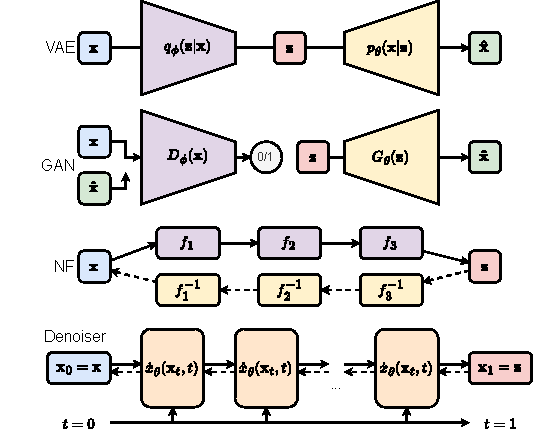
\includegraphics[width=0.8\textwidth]{Figures/transformers/pgms.pdf}
    \caption{An overview of the generative models covered in this thesis.}
    \label{fig:generative_models}
\end{figure}


\section{Older PGMs}

Over the course of this thesis the field of generative models has seen rapid development.
At the start of this thesis, two models dominated the field: Variational Autoencoders~\cite{AutoEncodingVariationalBayes} (VAEs) and GANs~\cite{GenerativeAdversarialNetworks}.
While these older models, especially GANs, produced very impressive results in select domains, the generation quality and fine control of the samples that we see today was not possible.
The current landscape of text-to-image~\cite{Imagen, Dalle, SD3}, and even text-to-video~\cite{ImagenVideo} generation would have been inconceivable just a few years ago.
While it is remarkable how quickly focus of these models has moved on, specifically to denoisers, it is still important to highlight them here, both for historical context and to understand the strengths of the models that have replaced them.

\subsection{Variational Autoencoders}

VAEs were introduced in 2013~\cite{AutoEncodingVariationalBayes} and quickly became a popular model for generative tasks, unsupervised learning and variational inference.
A VAE is an example of a latent variable model.
Here one introduces a latent random variable $\Z \in \mathcal{Z}$ which one marginalizes over to obtain the distribution of the data,
\begin{equation}
    p_\X(\x) = \int p_{\X,\Z}(\x, \z)\diff\z = \int p_\X(\x|\z)p_\Z(\z)\diff\z.
\end{equation}
The latent space usually covers all real values, $\mathcal{Z} = \mathbb{R}^d$, and the prior $p_\Z(\z)$ is taken to be a simple distribution, such as a diagonal Gaussian $\normal$.
Practically we would like to not enforce what information is stored in the latent variable.
The standard choice for modelling the likelihood is to use a parametrised Gaussian with constant variance,
\begin{equation}
    p_\X(\x|\z) \approx p_{\theta}(\x|\z) = \mathcal{N}(\x; G_{\theta}(\z), \sigma^2 I),
\end{equation}
where $G_{\theta}$ is a neural network called the decoder.

VAEs introduce an additional parametrized distribution to approximate the posterior which is also taken to be Gaussian with a diagonal covariance matrix,
\begin{equation}
    p_\Z(\z|\x) \approx q_\phi(\z|\x) = \mathcal{N}(\z; \boldsymbol{\mu}_\phi(\x), \boldsymbol{\Sigma}_\phi(\x)).
\end{equation}
Here the estimation of the mean and variance of the approximate posterior is done by a neural network called the encoder and gradients are backpropagated through the stochastic latent variable using the reparameterisation trick~\cite{AutoEncodingVariationalBayes}.

One can not train this model by simply maximizing the likelihood of the data, as the likelihood is intractable.
However, this form sets up a mapping between the data space to the latent space and back again and one can train the model by maximizing the evidence lower bound (ELBO).
Practically this involves minimizing two terms, the reconstruction loss and the KL-divergence between the approximate posterior and the prior,
\begin{equation}
        \mathcal{L}(\theta, \phi) = \mathbb{E}_{\z \sim q_{\phi}(\z|\x)}[||\x - G_{\theta}(\z)||^2] - \beta D_{KL}(q_{\phi}(\z|\x) || p_\Z(\z)),
\end{equation}
where $\beta$ is a hyperparameter that balances the two terms~\cite{BetaVAE}.

Typically the dimensionality of the latent space is much lower than the data space, so the information bottleneck means the model is forced to learn a compressed representation.
VAEs are simple to train but have a number of limitations.
The bottleneck means that the samples are often of low quality and lacking in high frequency detail.
The model is also sensitive to the tuning of $\beta$, often leading to a collapse into one of two regimes.
Either the prior loss dominates, all samples are encoded to the unit Gaussian and all information is lost.
Alternatively the reconstruction loss dominates, the posterior is non-Gaussian and extra steps are required to sample from it, such as fitting a kernel density estimator to the empirical distribution of the latent variables~\cite{KDEVAE}.

Conditional information can be injected into the VAE simply by combining the context variable with both the inputs to the encoder and decoder.
The compression of the latent means that it only stores orthogonal information to the context variable, which is useful for disentanglement~\cite{cVAE}.

VAEs were never particularly good at generating high quality samples, but they attempts were still made in HEP to use them for fast simulation of detector responses~\cite{VariationalAutoencodersJet, GraphVariationalAutoencoder, ParticlebasedFastJet}.
One other notable usecase for anomaly detection~\cite{VariationalAutoencodersAnomalous, DeepSetVAE, MassiveIssueAnomaly}.
Both of these applications produced mixed results and the field at large has moved on to more powerful models.


\subsection{Generative Adversarial Networks}

Up until recently, GANs were the state-of-the-art in generative models for producing high quality samples.
This was most notably demonstrated in the generation of high resolution images~\cite{StyleGAN2,StyleGAN3}.
GANs are based on a two-player min-max game between a generator $G_\theta(\z)$ and a discriminator $D_\phi(\x)$, each neural networks with parameters $\theta$ and $\phi$ respectively.
These networks contest with each other in a zero-sum game where the one network's loss is the other's gain.

The generator takes a random latent sample $\z \sim p_\Z(\z)$ and returns a synthetic sample $\hat{\x} = G_\theta(\z) \in \mathcal{X}$.
The discriminator takes samples from both the training set and the synthetic samples and returns a probability that the sample is from the training set, $D_\phi(\x) \in [0, 1]$.
The objective of the generator is to fool the discriminator into thinking the generated samples are real.
Given powerful enough networks, the unique Nash equilibrium of this game is a generator that produces the true data distribution and a uniform discriminator output for all real samples.

There are many variations for defining the specifics of this game and the loss functions, but arguably the most widely used is the original non-saturating loss~\cite{GenerativeAdversarialNetworks}.
This loss requires two passes through each network, one to update the discriminator and one to update the generator.
\begin{align}
    \mathcal{L}_{\text{D}}(\phi) &= -\mathbb{E}_{\x \sim \mathcal{D}}[\log D_{\phi}(\x)] - \mathbb{E}_{\z \sim p_\Z(\z)}\log(1 - D_{\phi}(G_{\theta}(\z))], \\
    \mathcal{L}_{\text{G}}(\theta) &= -\mathbb{E}_{\z \sim p_\Z(\z)}[\log D_{\phi}(G_{\theta}(\z))].
\end{align}
Other variants exist which use different loss derivations, such as the Wasserstein GAN~\cite{WGAN1} and the Geometric GAN~\cite{GeometricGAN}.
There is plenty of literature on which variants are best suited for different tasks and which actually converge to the desired Nash equilibrium~\cite{WhichTrainingMethods}.

The main difficulty of GANs is that they are difficult to train.
Often there is mode collapse, where the generator exploits some weakness in the discriminator and reproduces the same samples over and over.
Many tricks are required to stabalize training~\cite{WhichTrainingMethods}, such as minibatch discrimination~\cite{ProGAN} and gradient penalties~\cite{WGAN}.
Another drawback to GANs is that it is difficult to product a conditional generator $G_\theta(\x|\con)$.
Simply concatenating the context variable to both the generator and discriminator inputs leads to mixed results and the generator is prone to ignoring the context variable~\cite{cGAN}.

In HEP, GANs have mainly been trialed as a method for fast simulation~\cite{MPGAN, GAPT, CaloGAN, EPICGAN}.
However, the main issue is that GANs tend to not cover the full data distribution, and that most of the generation we are looking for in fast simulation is conditional;
detector response depends on the properties of the incoming particle, making GANs not optimal for this task.

\section{Normalizing Flows}

NFs are a popular tool for both variational inference~\cite{VariationalInferenceNormalizing}
and density estimation~\cite{NICENonlinearIndependenta}.
Like GANs and VAEs, they prescribe a method to train a transformation from a simple latent distribution into one that matches the data.
However, unlike GANs and VAEs, normalizing flows allow for explicit likelihood evaluation, making them well suited for density estimation.

Like all latent variable models, NFs turn a simple latent distribution into a complex data distribution.
However, NFs strive to do this exactly via the change of variables formula.
Given two random variables of equal dimensionality $\X$ and $\Z$ related by a bijective function $f: \mathcal{X} \rightarrow \mathcal{Z}$, the probability densities $p_\X(\x)$ and $p_\Z(\z)$ are related by
\begin{equation}
    \label{eq:change_of_variables}
    p_\X(\x) = p_\Z(f(\x)) \left|\det D f(\x) \right|.
\end{equation}
Here $f(\x)$ is a differentiable bijective function with a differentiable inverse, otherwise known as a diffeomorphism, and $D f(\x)$ is the Jacobian of the transformation.
The density $p_\X(\x)$ is called a \textit{pushforward} of the density $p_\Z(\z)$ by the function $f$, $p_\X = f_\# p_\Z$.

Unlike GANs, a NF constructs an explicit approximation of data density by defining it as a pushforward of a simple latent distribution, typically Gaussian, through a parametrized neural network,
\begin{equation}
    p_{\X}(\x) \approx p_{\theta}(\x) = f_{\theta \#} p_\Z(\z).
\end{equation}
Like all neural networks, NFs are built from the composition of several simple layers, but unlike other neural networks, each \textit{flow layer} has to be a diffeomorphism.
This is because the composition of two diffeomorphisms is itself a diffeomorphism, furthermore the Jacobian of the full transformation is simply the product of the Jacobians of the individual layers,
\begin{equation}
    f = f_1 \circ f_2 \circ \ldots \circ f_L \quad \Rightarrow \quad \det D f(\x) = \prod_{i=1}^L \det D f_i(\x_i).
\end{equation}
This composition property allows us to construct arbitrarily complex transformations, allowing for the approximation of any data distribution no matter how complex given a simple latent distribution~\cite{bogachev2005triangular}.

NFs are typically trained via a maximum log-likelihood approach, or more specifically, they use a negative log-likelihood loss function,
\begin{equation}
    \label{eq:nf_loss}
    \begin{aligned}
        \mathcal{L}(\theta)
        \frach &= \mathbb{E}_{\x \sim \mathcal{D}}[-\log p_{\theta}(\x)] \\
        \frach &= \mathbb{E}_{\x \sim \mathcal{D}}\left[-\log p_{\Z}(f_{\theta}(\x)) - \log \left|\det D f_{\theta}(\x) \right|\right] \\
        \frach &= \mathbb{E}_{\x \sim \mathcal{D}}\left[-\log p_{\Z}(f_{\theta}(\x)) - \sum_{i=1}^L \log \left|\det D f_i(\x_i) \right|\right].
    \end{aligned}
\end{equation}
Note that due to the composition property of the Jacobian, the log determinant term is a sum of the log determinants of the individual layers, leading to essentially independant terms in the final loss.

During training, the flow is said to run in forward mode, transforming samples from the data space to the latent space.
Once the model is trained, it can be used in forward mode to yield the density at any measured point, or it could be run in reverse mode $f^{-1}$, transforming samples from the latent space to the data space.

How to construct these

% How to construct a normalising flow with these layers
% Must be invertible
% Must be differentiable
% But to make it practical
% But ideally, it should be easy to compute the determinant of the jacobian
% It should be quick to compute the inverse
% Designing these flow layers is the core research problem in normalising flows


Important to note that if modelling discrete data, we need to dequantise the data
Singularities
Easiest method is to add noise to the data
Can be done variationally

Can learn conditional normalising flows through injection of context in each layers
Shown to match the aleatoric uncertainty in the data

\subsection{Linear Flows}
$f(x) = Ax + b$
inverse is $x = A^{-1}(z - b)$
Determinant is $|det(A)|$
Problem: inexpressive, determinant is $O(d^3)$

Can restrict the form of the matrix to make it easier,
Full - $O(d^3)$
Diagonal - $O(d)$
Triangular - $O(d^2)$
Block Diagonal - $O(c^2d)$
LU Factorised - $O(d^2)$
Spacial convolusion - $O(d)$
1x1 Convolusion - $O(d)$

\subsection{Coupling Flows}

General approach to construct non-linear flows
Partition the input into two parts
One part is passed through a neural network, two operations
$f(x) = (x_A, g(x_B | h(x_A)))$
g has to be invertible and simple to calculate
But there are no restrictions on h
Show diagram of coupling flow

Jacobian of the transformation is a block matrix
Can ignore the bottom left block in calculating the determinant
This means that we can have an arbitrarily complex h, MLP, CNN, etc

It is important to permute or use a linear transformation between coupling layers to
maximise the expressiveness of the model.

Popular coupling transformes include nice additive
RealNVP, scale and shift
Splines are the most expressive

\subsection{Autoregressive Flows}

Autoregressive models $p(x) = \prod_i p(x_i | x_{<i})$
Require defining a specific ordering of the variables

Sampling is sequential and slow
Can use inverse for training, which means training is slow
Jacobian is triangular and easy to compute


\section{Denoising Models}



\subsection{Score-Based Generative Models}

\subsection{Flow Matching}

\subsection{Consistency Models}
